\documentclass[12pt]{article}
\usepackage[paper=letterpaper,margin=2cm]{geometry}
\usepackage{amsmath,amssymb,amsfonts}
\usepackage{newtxtext,newtxmath}
\usepackage{enumitem}
\usepackage{titling}
\usepackage{subfig,graphicx}
\usepackage[colorlinks=true]{hyperref}
\usepackage{multirow}
\usepackage{listings}
\usepackage{xcolor}
\usepackage{float}

\definecolor{codegreen}{rgb}{0,0.6,0}
\definecolor{codegray}{rgb}{0.5,0.5,0.5}
\definecolor{codepurple}{rgb}{0.58,0,0.82}
\definecolor{backcolour}{rgb}{0.95,0.95,0.92}

\newcommand{\ind}{\perp\!\!\!\perp}

\lstdefinestyle{mystyle}{
    commentstyle=\color{codegreen},
    keywordstyle=\color{magenta},
    numberstyle=\tiny\color{codegray},
    stringstyle=\color{codepurple},
    basicstyle=\ttfamily\footnotesize,
    breakatwhitespace=false,
    breaklines=true,
    captionpos=b,
    keepspaces=true,
    numbers=left,
    numbersep=5pt,
    showspaces=false,
    showstringspaces=false,
    showtabs=false,
    tabsize=2
}
\lstset{style=mystyle}

\begin{document}

\begin{center}
\large{Aprendizagem 2023}\\
Homework II -- Group 28\\
\vskip 0.3cm
Gonçalo Bárias (ist1103124) \& Raquel Braunschweig (ist1102624)\vskip 1cm

\large{\textbf{Part I}: Pen and Paper}\normalsize
\end{center}

\noindent Consider the following dataset ($y_3$ - $y_5$ are all categorical variables and the domain of $y_2$ is $[0,1]$):

\begin{figure}[H]
    \centering
    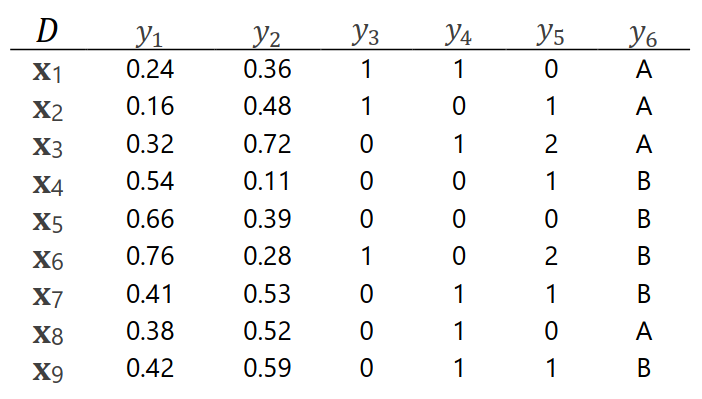
\includegraphics[width=9cm]{./assets/dataset_d.png}
    \label{fig:PartI-dataset-d}
\end{figure}

\begin{enumerate}[leftmargin=\labelsep]
    \item \textbf{Consider $x_1$ - $x_7$ to be training observations, $x_8$ - $x_9$ to be testing observations, $y_1$ - $y_5$ to be input
          variables and $y_6$ to be the target variable.\\
          \textit{Hint}: you can use \texttt{scipy.stats.multivariate\_normal} for multivariate distribution calculus}
          \begin{enumerate}
          \item \textbf{Learn a Bayesian classifier assuming: i) $\{y_1, y_2\}$, $\{y_3, y_4\}$ and $\{y_5\}$ sets of independent
                variables (e.g., $y_1 \ind y_3$ yet $y_1 \not\!\ind y_2$), and ii) $y_1 \times y_2 \in \mathbb{R}^{2}$ is normally distributed. Show all
                parameters (distributions and priors for subsequent testing).}

          \vskip 0.3cm
          Gonçalo

          \item \textbf{Under a MAP assumption, classify each testing observation showing all your calculus.}

          \vskip 0.3cm
          Gonçalo

          \item \textbf{Consider that the default decision threshold of $\theta = 0.5$ can be adjusted according to}

                \[
                        f(\textbf{x}|\theta)=
                    \begin{cases}
                        A,& P(A|\textbf{x}) > \theta\\
                        B,& \text{otherwise}
                    \end{cases}
                \]

                \textbf{Under a maximum likelihood assumption, what thresholds optimize testing accuracy?}

          \vskip 0.3cm
          Raquel
          \end{enumerate}

    \item \textbf{Let $y_1$ be the target numeric variable, $y_2$ - $y_6$ be the input variables where $y_2$ is binarized under an
          equal-width (equal-range) discretization. For the evaluation of regressors, consider a 3-fold
          cross-validation over the full dataset ($x_1$ - $x_9$) without shuffling the observations.}
          \begin{enumerate}
          \item \textbf{Identify the observations and features per data fold after the binarization procedure.}

          \vskip 0.3cm
          
          To do the \textbf{binarization procedure} with an \textbf{equal-width discretization}, we need to find the range of values
            for $y_2$ and then divide it into two intervals. Bellow are the calculations of the intervals:


          \begin{center}
            $y_2$ ranges from 0.11 to 0.72 
          \end{center}

          \textbf{Therefore}, the width shall be:

          \begin{equation*}
            width = \frac{0.72 - 0.11}{2} = 0.305
          \end{equation*}

          \textbf{Now,} we can finally separate $y_2$ into two intervals:

          \begin{equation*}
            interval_1 = [0.11, 0.11 + 0.305] = [0.11, 0.415]
          \end{equation*}

          \begin{equation*}
            interval_2 = [0.72 - 0.305, 0.72] = [0.415, 0.72]
          \end{equation*}

          \textbf{Here is the binazation of $y_2$} based on those intervals:
          \begin{center}
            \begin{tabular}{c|cccccc}
                \(D\) & \(y_1\) & \(y_2\) & \(y_3\) & \(y_4\) & \(y_5\) & \(y_6\)\\
                \hline
                \(x_1\) & 0.24 & 0 & 1 & 1 & 0 & A  \\
                \(x_2\) & 0.16 & 1 & 1 & 0 & 1 & A  \\
                \(x_3\) & 0.32 & 1 & 0 & 1 & 2 & A  \\
                \(x_4\) & 0.54 & 0 & 0 & 0 & 1 & B  \\
                \(x_5\) & 0.66 & 0 & 0 & 0 & 0 & B  \\
                \(x_6\) & 0.76 & 0 & 1 & 0 & 2 & B  \\
                \(x_7\) & 0.41 & 1 & 0 & 1 & 1 & B  \\
                \(x_8\) & 0.38 & 1 & 0 & 1 & 0 & A  \\
                \(x_9\) & 0.42 & 1 & 0 & 1 & 1 & B  \\
            \end{tabular}
          \end{center}

          \textbf{The next step} is identifying our folds, which will be:
          \begin{center}
            Fold 1 = $x_1$ $x_2$ $x_3$  \\
            Fold 2 = $x_4$ $x_5$ $x_6$ \\
            Fold 3 = $x_7$ $x_8$ $x_9$ \\
          \end{center}

          \textbf{So} our datasets will be:

          \begin{center}
            \textbf{Fold 1} \\
            \begin{tabular}{c|cccccc}
                \(D\) & \(y_1\) & \(y_2\) & \(y_3\) & \(y_4\) & \(y_5\) & \(y_6\)\\
                \hline
                \(x_1\) & 0.24 & 0 & 1 & 1 & 0 & A  \\
                \(x_2\) & 0.16 & 1 & 1 & 0 & 1 & A  \\
                \(x_3\) & 0.32 & 1 & 0 & 1 & 2 & A  \\
            \end{tabular}
          \end{center}

          \begin{center}
            \textbf{Fold 2} \\
            \begin{tabular}{c|cccccc}
                \(D\) & \(y_1\) & \(y_2\) & \(y_3\) & \(y_4\) & \(y_5\) & \(y_6\)\\
                \hline
                \(x_4\) & 0.54 & 0 & 0 & 0 & 1 & B  \\
                \(x_5\) & 0.66 & 0 & 0 & 0 & 0 & B  \\
                \(x_6\) & 0.76 & 0 & 1 & 0 & 2 & B  \\
            \end{tabular}
          \end{center}

          \begin{center}
            \textbf{Fold 3} \\
            \begin{tabular}{c|cccccc}
                \(D\) & \(y_1\) & \(y_2\) & \(y_3\) & \(y_4\) & \(y_5\) & \(y_6\)\\
                \hline
                \(x_7\) & 0.41 & 1 & 0 & 1 & 1 & B  \\
                \(x_8\) & 0.38 & 1 & 0 & 1 & 0 & A  \\
                \(x_9\) & 0.42 & 1 & 0 & 1 & 1 & B  \\
            \end{tabular}
          \end{center}

    \item \textbf{Consider a distance-weighted \textit{k}NN with k = 3, Hamming distance (\textit{d}), and 1 / \textit{d} weighting.
          Compute the MAE of this \textit{k}NN regressor for the $1^{st}$ iteration of the cross-validation (i.e. train
          observations have the lower indices).}

          \vskip 0.3cm

          The formula for \textbf{weighted average} is the following:

          \begin{equation}\label{exI2-a-WA}
            \text{Weighted Average} = \frac{{\frac{1}{{d_1}} \cdot y_1 + \frac{1}{{d_2}} \cdot y_2 + \frac{1}{{d_3}} \cdot y_3}}{{\frac{1}{{d_1}} + \frac{1}{{d_2}} + \frac{1}{{d_3}}}}
          \end{equation}

          
          The formula for the \textbf{mean absolute error} is given by:

          \begin{equation}\label{exI2-a-MAE}
              MAE = \frac{1}{n} \sum_{i=1}^{n} \left| y_i - \hat{y}_i \right|     
          \end{equation}

          As stated in the prompt, we will use Folds 1 and 2 for training, reserving Fold 3 for testing. Let's start by computing
           the \textbf{Hamming distances}, for $x_7$ first:

           \begin{center}
            \begin{tabular}{c|cccccc}
                \(H(x_7,x_j)\)& \(x_1\) & \(x_2\) & \(x_3\) & \(x_4\) & \(x_5\) &\(x_6\) \\
                \hline
                               & 4 & 3 & 2 & 2 & 3 & 4 \\
            \end{tabular}
          \end{center}
          

          \textbf{Now,} for $x_8$:

          \begin{center}
            \begin{tabular}{c|cccccc}
                \(H(x_8,x_j)\)& \(x_1\) & \(x_2\) & \(x_3\) & \(x_4\) & \(x_5\) &\(x_6\) \\
                \hline
                               & 2 & 3 & 1 & 4 & 3 & 5 \\
            \end{tabular}
          \end{center}

          \textbf{Finally,} for $x_9$:

          \begin{center}
            \begin{tabular}{c|cccccc}
                \(H(x_9,x_j)\)& \(x_1\) & \(x_2\) & \(x_3\) & \(x_4\) & \(x_5\) &\(x_6\) \\
                \hline
                               & 4 & 3 & 2 & 2 & 3 & 4 \\
            \end{tabular}
          \end{center}

          Now let's determine the \textbf{three closest neighbors} to each test observation:
          
          \begin{itemize}
            \item For $x_7$ it is $x_2$, $x_3$ and $x_4$
            \item For $x_8$ it is $x_1$, $x_2$ and $x_3$
            \item For $x_9$ it is $x_2$, $x_3$ and $x_4$
          \end{itemize}

          The next step is calculating their \textbf{weighted average}, replacing by the
           formula on \eqref{exI2-a-WA}, we get the following values:
            
          \begin{center}
            Weighted average for $x_7$ = 0.37375 \\
            Weighted average for $x_8$ $\approx$ 0.26909 \\
            Weighted average for $x_9$ = 0.37375 \\
          \end{center}
          
          \textbf{Finally,} let's compute the mean absolute error by using the equation 
           on \eqref{exI2-a-MAE}:

           \begin{equation*}
            MAE = 0.06447
           \end{equation*}

          \end{enumerate}
\end{enumerate}

\vskip 0.5cm

\begin{center}
\large{\textbf{Part II}: Programming and critical analysis}\normalsize
\end{center}

\noindent Considering the \texttt{column\_diagnosis.arff} dataset available at the course webpage’s homework tab. Using \texttt{sklearn}, apply a 10-fold stratified
cross-validation with shuffling (\texttt{random\_state=0}) for the assessment of predictive models along this section.

\begin{enumerate}[leftmargin=\labelsep]
    \item \textbf{Compare the performance of \textit{k}NN with k = 5 and Naïve Bayes with Gaussian assumption
          (consider all remaining parameters for each classifier as \texttt{sklearn}'s default):}
          \begin{enumerate}
          \item \textbf{Plot two boxplots with the fold accuracies for each classifier.}

          \vskip 0.3cm
          \lstinputlisting[language=Python]{./assets/code_1a.py}

          \begin{figure}[H]
            \centering
            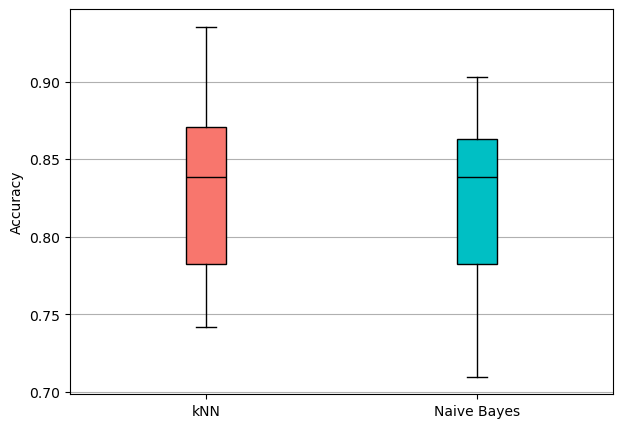
\includegraphics[width=13cm]{./assets/boxplot_ex1_PartII.png}
            \caption{Boxplots with the fold accuracies of \textit{k}NN (k = 5) and Naïve Bayes}
            \label{fig:PartII-ex1a}
          \end{figure}

          \item \textbf{Using \texttt{scipy}, test the hypothesis "\textit{k}NN is statistically superior to Naïve Bayes regarding
                accuracy", asserting whether is true.}

          \vskip 0.3cm
          We'll consider the null hypothesis and alternate hypothesis below and perform a single-tailed test using the accuracies
          obtained in the previous answer,

          $$
              \begin{aligned}
                  H_0: & \quad\text{accuracy}_{k\text{NN}} = \text{accuracy}_{\text{Naïve Bayes}} \\
                  H_1: & \quad\text{accuracy}_{k\text{NN}} > \text{accuracy}_{\text{Naïve Bayes}}
              \end{aligned}
          $$

          \lstinputlisting[language=Python]{./assets/code_1b.py}

          Using \texttt{scipy} we get a p-value of, approximately, 0.190428 = 19.0428 \%.

          This means we cannot reject the hypothesis $H_0$ at common significance levels (1\%, 5\% and 10\%).

          \textbf{Therefore,} we cannot assert that \textit{k}NN is statistically superior to Naïve Bayes. We also cannot
          state that the hypothesis on the statement is outright false without checking other statistical tests.
          \end{enumerate}

    \item \textbf{Consider two \textit{k}NN predictors with k = 1 and k = 5 (uniform weights, Euclidean distance,
          all remaining parameters as default). Plot the differences between the two cumulative confusion
          matrices of the predictors. Comment.}

          \vskip 0.3cm
          \lstinputlisting[language=Python]{./assets/code_2.py}

          \begin{figure}[H]
              \centering
              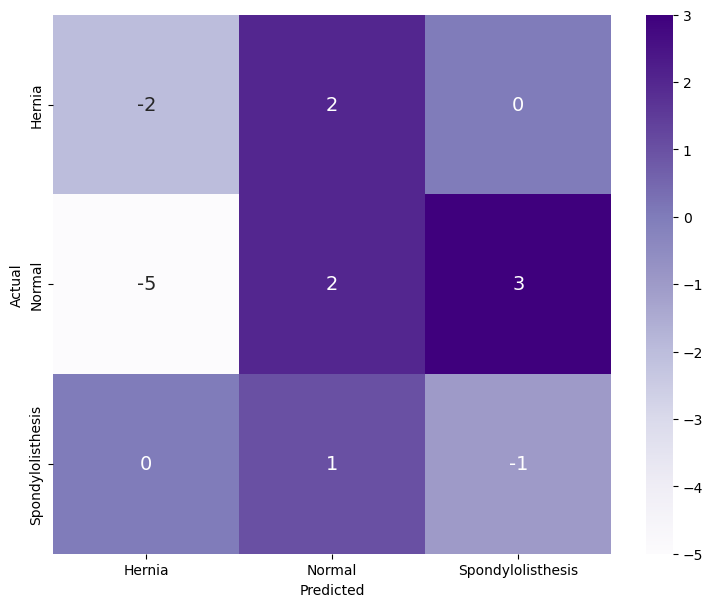
\includegraphics[width=13cm]{./assets/cummulative_heatmap_ex2_PartII.png}
              \caption{Confusion Matrix Differences Between k=1 and k=5 k-Nearest Neighbors (\textit{k}NN) Classifiers}
              \label{fig:PartII-ex2}
          \end{figure}

          Blah % TODO: Need to comment the plot

    \item \textbf{Considering the unique properties of \texttt{column\_diagnosis}, identify three possible difficulties
          of Naïve Bayes when learning from the given dataset.}

          \vskip 0.3cm
          Here are three possible difficulties of Naïve Bayes when learning from the given dataset,
          in no particular order:

          \begin{itemize}
              \item Variable dependencies (inadequacy of independence assumption).
              \item Variables not normally distributed (inadequacy of Gaussian assumption). Probability estimates from a limited number of observations (e.g., inadequate estimates, null probabilities).
              \item Imbalanced class creating biases in MAP estimates via priors.
          \end{itemize}
\end{enumerate}

\end{document}
